\documentclass[ngerman]{article}

\usepackage{xcolor}
\usepackage[T1]{fontenc}
\usepackage{pgffor}
\usepackage{todonotes}
\usepackage{minted}
\usepackage{graphicx}
\usepackage{minted}
\usemintedstyle{vs}
\usepackage{fancyhdr}
\usepackage{hyperref}
\usepackage{tcolorbox}
\usepackage{etoolbox}
\usepackage[margin=1.2in]{geometry}
\usepackage[ngerman]{babel} 
\usepackage{inconsolata}
\usepackage{bookmark}
\usepackage{wrapfig} 
\usepackage{lipsum}
\usepackage[autolang=other, backend=biber]{biblatex}
\addbibresource{refs.bib}

\hypersetup{
  colorlinks=true,
  linkcolor=blue,
  filecolor=magenta,
  citecolor=blue,
  urlcolor=blue,
}

\renewcommand*\familydefault{\ttdefault} %% Only if the base font of the document is to be typewriter style

\newcommand{\topic}[1]{\tcbox[on line,arc=4pt,colframe=white,boxrule=0pt,boxsep=0pt,left=4pt,right=4pt,top=3pt,bottom=2pt,colback=gray!30]{#1}}

\newcommand{\br}{\linebreak\linebreak}

\newcommand{\link}[2][]{%
    \ifblank{#1}{%
        \hyperref[sec:#2]{#2}%
    }{%
        \hyperref[sec:#1]{#2}%
    }%
}

\newenvironment{code}
  {%
    \begin{tcolorbox}[
        colback=white,
        colframe=black,
        boxrule=0.5pt,
        arc=4pt,
        left=2mm,
        right=2mm,
        top=2mm,
        bottom=2mm,
      ]
      }{% 
    \end{tcolorbox}
    }


\newcommand{\cmt}[1]{\textcolor{gray!60}{\textit{/* #1 */}}}

\newcommand{\qt}[1]{„#1“}

% Define a custom command for colored boxes around words
\newcommand{\topics}[1]{%
  \linebreak
  \linebreak
  \foreach \word in {#1} {%
    \topic{\word}%
  }%
  \linebreak
}


\title{Bachelorarbeit}
\author{Max Richter}

\begin{document}

\pagestyle{fancy}
\fancyhead{} % clear all header fields
\fancyhead[RO,LE]{\textbf{WebAssembly-basierte visuelle Programmiersprache}}
\fancyfoot{} % clear all footer fields
\fancyfoot[LE,RO]{\thepage}
\fancyfoot[LO,CE]{\href{https://github.com/jim-fx/bachelor}{github.com/jim-fx/bachelor}}
\fancyfoot[CO,RE]{Max Richter}

\raggedright

\maketitle
\pagebreak

\tableofcontents

\pagebreak

\section{Einleitung}
In unserer heutigen digitalisierten Welt spielen Human-Computer Interfaces (HCI's) eine entscheidende Rolle.
Hierbei gibt es eine weite Spanne von Komplexität, von einfach zu bedienenden grafischen Benutzeroberflächen bis zu komplexen Programmiersprachen. 

Da Menschen Konzepte und Relationen größtenteils visuell und räumlich verarbeiten \cite{smith1975pygmalion}, bieten visuelle Programmiersprachen (VPL's) einen guten Mittelweg für programmierunerfahrene Nutzer*innen. 
 
Sie vereinen die Benutzerfreundlichkeit grafischer Interfaces mit der Komplexität und Flexibilität textbasierter Programmiersprachen. 

\subsection{Hintergrund}
\subsection{Problemstellung}
\subsection{Zielsetzung}
\subsection{Forschungsfragen}

Inwieweit eignet sich WebAssembly als Grundlage für eine node-basierte visuelle Programmiersprache?  
\linebreak
\linebreak
Welche Auswirkungen haben die spezifischen Vor- und Nachteile von WebAssembly auf die Realisierbarkeit, Funktionalität, Nutzerfreundlichkeit, Performance, Flexibilität und Robustheit einer solchen Programmiersprache?

\section{Theoretischer Rahmen}

\subsection{Definition von visuellen Programmiersprachen}
Eine visuelle Programmiersprache stellt die Komponenten und Verbindungen eines Programms in mehr als einer Dimension dar. Oft ist diese Dimension eine zweidimensionale Fläche auf der die einzelnen Funktionen oder Komponenten eines Systems visuell dargestellt werden. \cite{Myers}
Auch wenn textuelle Sprache auf einer zweidimensionalen Oberfläche dargestellt wird, so ist sie meist aus Sicht des Interpreters oder Compilers ein eindimensionaler Stream aus Tokens.

\subsection{Klassifikation von visuellen Programmiersprachen}

Nach Burnett\&Mayer können VPL's in 5 verschiedenen Klassen eingeteilt werden \cite{BURNETT1994287}. Diese einzelnen Klassen schließen sich nicht gegenseitig aus und können auch in Kombination verwendet werden.

\subsubsection{\qt{Purely visual languages}}
Purely visual languages haben keine textuelle Repräsentation und sind ausschließlich visuell. Ein Beispiel hierfür ist \textit{Scratch}, das es Nutzern ermöglicht, durch das Zusammensetzen von Blöcken Programme zu erstellen, ohne eine einzige Zeile Code zu schreiben.


\subsubsection{\qt{Hybrid text and visual systems}}
Hybrid text and visual systems haben eine textuelle Repräsentation, die parallel zur visuellen Repräsentation existiert. Ein Beispiel hierfür ist \textit{Microsoft's Visual Programming Language}, das Teil von Microsoft Robotics Developer Studio ist und eine hybride Umgebung bietet, in der Nutzer sowohl Code schreiben als auch visuelle Elemente nutzen können.

\subsubsection{\qt{Programming-by-example Systems}}
Programming-by-example systems erlauben es dem Nutzer, ein Programm zu schreiben, indem er die gewünschte Funktionalität in einem Beispiel demonstriert. \textit{Etoys}, basierend auf Squeak, ist ein Beispiel für ein solches System, bei dem Benutzer durch das Demonstrieren von Aktionen Objekte programmieren können.

\subsubsection{\qt{Constraint-oriented Systems}}
Constraint-oriented Systems erlauben es dem Nutzer, Constraints zwischen den Komponenten des Programms zu definieren. \textit{ThingLab} ist ein Beispiel für ein constraint-orientiertes System, das dem Benutzer ermöglicht, durch die Definition von Einschränkungen zwischen Objekten interaktive Simulationen zu erstellen.

\subsubsection{\qt{Form-based systems}}
Form-based systems erlauben es dem Nutzer, Programme zu schreiben, indem er Formen ausfüllt. Ein klassisches Beispiel für ein formbasiertes System ist \textit{Oracle Forms}, das eine GUI für Datenbankabfragen und -transaktionen bietet, indem es Benutzern ermöglicht, Formulare auszufüllen, die dann in SQL-Code umgewandelt werden.

\subsection{Historische Vorbilder}

\subsubsection{SketchPad (1963)}
\label{sec:SketchPad}
\begingroup
\setlength\intextsep{2pt}
\begin{minipage}{\linewidth}
\begin{wrapfigure}{R}{0.3\textwidth}
  \centering
  \includegraphics[width=0.3\textwidth]{./graphics/sketchpad-sutherland.jpg} % Change example-image-a with your image filename
  \caption{SketchPad \cite{sutherlandSketchpad}}
\end{wrapfigure}
SketchPad ist ein von Ivan Sutherland entwickeltes Programm das 1963 am MIT veröffentlicht wurde. 
SketchPad benutzte einen Lightpen als Eingabegerät und war das erste Programm, das die Interaktion mit einem Computer über eine grafische Benutzeroberfläche ermöglichte. 
Es erlaubte den Nutzer*innen, geometrische Formen auf einem Bildschirm zu zeichnen und diese zu manipulieren.
  Dabei existierten diese Formen auf einem virtuellen \qt{Papier}, dass der Nutzer bewegen und zoomen konnte. Dieses Konzept von bewegen und Zoomen virtueller Oberflächen war revolutionär für die damalige Zeit.
  Dies wird deutlich durch den Fakt das der Präsentator während der Präsentation von SketchPad \cite{sketchpadDemo} (10:30) keine Worte fand, um diesen Vorgang zu beschreiben.
Ein weiteres Feature war die Möglichkeit, Constraints zwischen den Formen zu definieren, ähnlich wie in modernen CAD-Programmen. 
Wenn man sich die Videodemo von SketchPad anschaut fallen viele Paradigmen auf, die wir heute als gegeben ansehen.
\linebreak
\linebreak
Auch wenn SketchPad nicht direkt in die Definition einer VPL passt, war es ein Meilenstein der Entwicklung von grafischen HCI's. Was durch die Verleihung des Turing Awards an Ivan Sutherland 1988 bestätigt wurde.
\end{minipage}
\endgroup

\subsubsection{Pygmalion (1970)}
\begingroup
\setlength\intextsep{2pt}
\begin{minipage}{\linewidth}
\begin{wrapfigure}{L}{0.4\textwidth}
  \centering
  \includegraphics[width=0.4\textwidth]{./graphics/pygmalion.jpg} % Change example-image-a with your image filename
  \caption{Fakultät in Pygmalion \cite{smith1975pygmalion}}
  \label{fig:pygmalion_demo}
\end{wrapfigure}

Pygmalion ist eine visuelle Programmiersprache die um 1970 von David Canfield Smith im Rahmen seiner Doktorarbeit entwickelt wurde. Inspiriert wurde sie von der mythischen Figur des Bildhauers Pygmalion der seine Skulpturen zum Leben erwecken konnte.
Die Sprache erlangte nie eine große Verbreitung, war aber ein wichtiger Meilenstein in der Entwicklung von visuellen Programmiersprachen und HCI's.
Pygmalion wurde in Smalltalk implementiert und war eine der ersten visuellen Programmiersprachen. Über eine grafische Oberfläche konnten die Nutzer*innen Blöcke, Icons und Verbindungen erstellen und manipulieren im damit Programme zu definieren.
  Icons waren damals eine Neuerung und wurden von den Entwicklern als \qt{eine Art von visuellen Variablen} bezeichnet. 
  Die Sprache war eine der ersten Beispiele von \qt{Programming By Example} oder PBE.
Die Nutzer*innen konnten Programme schreiben, indem sie die gewünschte Funktionalität in einem Beispiel demonstrieren. 
In Abbildung \ref{fig:pygmalion_demo} wird auf diese Art die Fakultät einer Zahl berechnet. 

\end{minipage}
\endgroup

\subsubsection{Cube (1996)}

\begingroup
\setlength\intextsep{2pt}

\begin{minipage}{\linewidth}
\begin{wrapfigure}{R}{0.4\textwidth}
  \centering
  \includegraphics[width=0.4\textwidth]{./graphics/cube_vpl.png} % Change example-image-a with your image filename
  \caption{Datenfluss in Cube \cite{najork1996programming}}
  \label{fig:cube_demo}
\end{wrapfigure}
  \qt{Cube ist eine dreidimensionale, visuelle, statisch typisierte Programmiersprache höherer Ordnung, die für den Einsatz in einer auf virtueller Realität basierenden Programmierumgebung entwickelt wurde.}  \cite{najork1996programming}
In \textit{Cube} werden einzelne Funktionen als, wie der Name schon verrät, Würfel dargestellt. Die Nutzer*innen können dann diese Cubes miteinander verbinden, um Programme zu erstellen.
Canfield geht in seiner Arbeit spezifisch auf den Vergleich zu Rohren und Wasserfluss ein. Somit bedient sich \textit{Cube} einer für Menschen relativ intuitiven Darstellung von Wasserfluss durch Rohre, um den Datenfluss innerhalb des Programms darzustellen.
  Ein interessantes Detail hierbei ist, das diese \qt{Rohre} keine Richtung haben und Daten in beide Richtungen fließen können. 
Da \textit{Cube} eine höhere Programmiersprache ist, können die Cubes auch als Argumente an andere Cubes übergeben werden. Dies ermöglicht es, komplexe Programme zu erstellen, die aus vielen einzelnen Cubes bestehen. 
\linebreak
\linebreak
Dieses Konzept ist relevant für meine persönliche Arbeit, siehe \link[HON]{Higher Order Nodes}.

\end{minipage}
\endgroup
\pagebreak

\subsection{Node-basierte visuelle Programmiersprachen}
In meiner Recherche nach modernen VPL's habe ich mich spezifisch auf node-basierte VPL's konzentriert die entweder durch ihre Popularität oder ihre Spezifizierung relevant für diese Arbeit sind.

\subsubsection{Node-RED}

Node-RED ist eine webbasierte Programmier- und Ausführungsumgebung die auf Nodes basiert und es den Nutzern ermöglicht, diese Nodes miteinander zu verknüpfen, um \qt{Flows} zu erstellen. 
Es wurde 2013 von IBM entwickelt und ist seit 2016 teil der OpenJS Foundation (damals JS Foundation).
\cite{nodered}

\begin{figure}[htbp]
  \centering
  \includegraphics[width=0.7\textwidth]{./graphics/node-red-3_1_8.png}
  \caption{Node Red v3.1.8}
  \label{fig:node_red}
\end{figure}

Node-RED findet vor allem Anwendung in den Bereichen IoT und Home Automation, da es eine Vielzahl von Anbindungen an verschiedene Geräte und Dienste bietet. 
Node-RED ist ein Beispiel für sogenanntes datenstromorientierte Programmierung, bei dem die Daten durch die Nodes fließen und diese verarbeiten. Das heißt es gibt keine einmalige Ausführung, sondern das System kann kontinuierlich Daten verarbeiten und auf externe Events reagieren.

\pagebreak
\subsubsection{Blender}
Blender ist eine weitverbreitete open-source 3D Modellierungs- und Animationssoftware. Blender bietet node-basierte Interfaces zur Erstellung von Materialien, Texturen und Geometrien an. 
\cite{blender}
Nach ungefähr 8 Jahren persönlicher Erfahrung mit Blender im privaten und professionellen Umfeld hat diese Software meine Erfahrungen und Meinungen zu visuellen Node-Editoren maßgeblich geprägt.
Für diese Arbeit ist Blender relevant, da es sich auch mit dem Erstellen von 3D-Modellen beschäftigt.

\begin{figure}[htbp]
  \centering
  \includegraphics[width=0.7\textwidth]{./graphics/blender-shader.png}
  \caption{Blender 3.5 Shader Editor}
  \label{fig:blender-shader}
\end{figure}

Vor allem die User-Experience der Blender Node-Editoren ist ein großer Vorteil. So bietet Blender für die meisten oft benötigten Funktionen Shortcuts an, die es ermöglichen, schnell und effizient zu arbeiten.
Ähnlich wie in Node-RED ist der Datenfluss der westlichen Leserichtung angepasst, von links nach rechts. Dies ermöglicht es, den Datenfluss intuitiv zu verfolgen und zu verstehen.
\linebreak
\linebreak
% erklären wie der geometrz node editor nodes benutzt im higher order functions zu machen, wie z.b. loops caching simulationen etc.
Im Gegensatz zum Shader Editor (sieht Abbildung \ref{fig:blender-shader}) bietet der Geometry Node Editor die Möglichkeit komplexere Setups zu erstellen. So gibt es zum Beispiel \qt{Repeat Zones}  die es ermöglichen eine Gruppe von Nodes arbiträr oft zu wiederholen.

\begin{figure}[htbp]
  \centering
  \includegraphics[width=0.6\textwidth]{./graphics/modeling_geometry-nodes_repeat_zone.png}
  \caption{Blender 4.1 Repeat Zone}
  \label{fig:blender-repeat}
\end{figure}

\subsubsection{SpeedTree}

\subsection{WebAssembly}
WebAssembly (WASM) ist ein Bytecode-Format für eine Stack-basierte virtuelle Maschine. Es wurde von der WebAssembly Working Group des World Wide Web Consortium (W3C) entwickelt und ist seit 2017 ein offizieller Web-Standard \cite{Haas2017}. 
\linebreak
\linebreak
Es wird hauptsächlich als Kompilierungsziel für kompilierte Programmiersprachen wie C, C++ und Rust benutzt, um diese in Webanwendungen zu integrieren. Im Gegensatz zu Javascript ist WebAssembly nicht garbage-collected und ist außerdem stark typisiert. Dies ermöglicht es, performante und sicherere Anwendungen zu entwickeln.
\subsubsection{WASI}
\cmt{WebAssembly System Interface}
\subsubsection{WAT}
\cmt{WebAssembly Text Format}
\subsubsection{WebAssembly Component Model}
\cmt{Kind of like ES-Modules or C-Style Linking}
\subsubsection{WIT}
\cmt{WebAssembly Interface Types}

\section{Konzept}

\subsection{Anforderungen}

- Flexibilität

\ \ $\rightarrow$  Einfachheit


- Gute UX

\ \ $\rightarrow$ Geschwindigkeit


- gerne das die einzelnen komponenten nicht in derselben umgebung laufen müssen

- Ähnlich wie die Ziele von WASM

- Damit die einzelnen Komponenten in unterschiedlichen Umgebungen implementiert werden können

\subsection{Architektur}

Aus den vorher genannten Zielen ergeben sich folgende Anforderungen an die Architektur:

\begin{itemize}
  \item Geschwindigkeit
  \item Einfachheit
  \item Erweiterbarkeit
\end{itemize}

- drei unterschiedlich module. 

- Möglichst minimale interfaces. 

\subsubsection{Datentypen}

Die Datentypen wurden möglichst minimal gehalten. Dies dient zum einen dem Ziel das gesamte System so einfach und verständlich wie möglich zu halten, und zum
anderen macht es die Serialisierung und Deserialisierung der Daten schneller.
\linebreak
\linebreak
Die drei Hauptdatentypen sind \link[Node]{Node}, \link[data_node_type]{Node-Type} und \link[Node-Graph]{Node-Graph}. 

\begin{figure}[htbp]
  \begin{code}
    \begin{minted}{typescript}
type Node = {
  id: number;                     // Primäre ID der Node
  type: string;                   // Type der Node, bsp: max/plantarium/math
  props?: Record<string, any>,    // Daten der Node
  position: [x: number, y: number]
}
    \end{minted}
  \end{code}

  \caption{Datenstruktur einer \link[Node]{Node} (TypeScript)}
  \label{fig:data_node}

\end{figure}

\begin{figure}[htbp]
  \begin{code}
    \begin{minted}{typescript}
type NodeType = {
  id: string;
  inputs?: Record<string, NodeInput>
  outputs?: string[];
  execute?: (args: number[]) => unknown;
}
    \end{minted}
  \end{code}

  \caption{Datenstruktur des \link[Node-Typ]{Node-Typen} (TypeScript)}
  \label{sec:data_node_type}

\end{figure}

\begin{figure}[htbp]
  \begin{code}
    \begin{minted}{typescript}
type Graph = {
  id: number;                                 // Primäre ID des Graphen
  nodes: Node[];                              // Liste aller Nodes
  edges: [number, number, number, string][];  // Liste aller Verbindungen
}
    \end{minted}
  \end{code}

  \caption{Datenstruktur eines \link{Node-Graph} (TypeScript)}
  \label{fig:data_node_graph}

\end{figure}

\begin{figure}
    \centering
    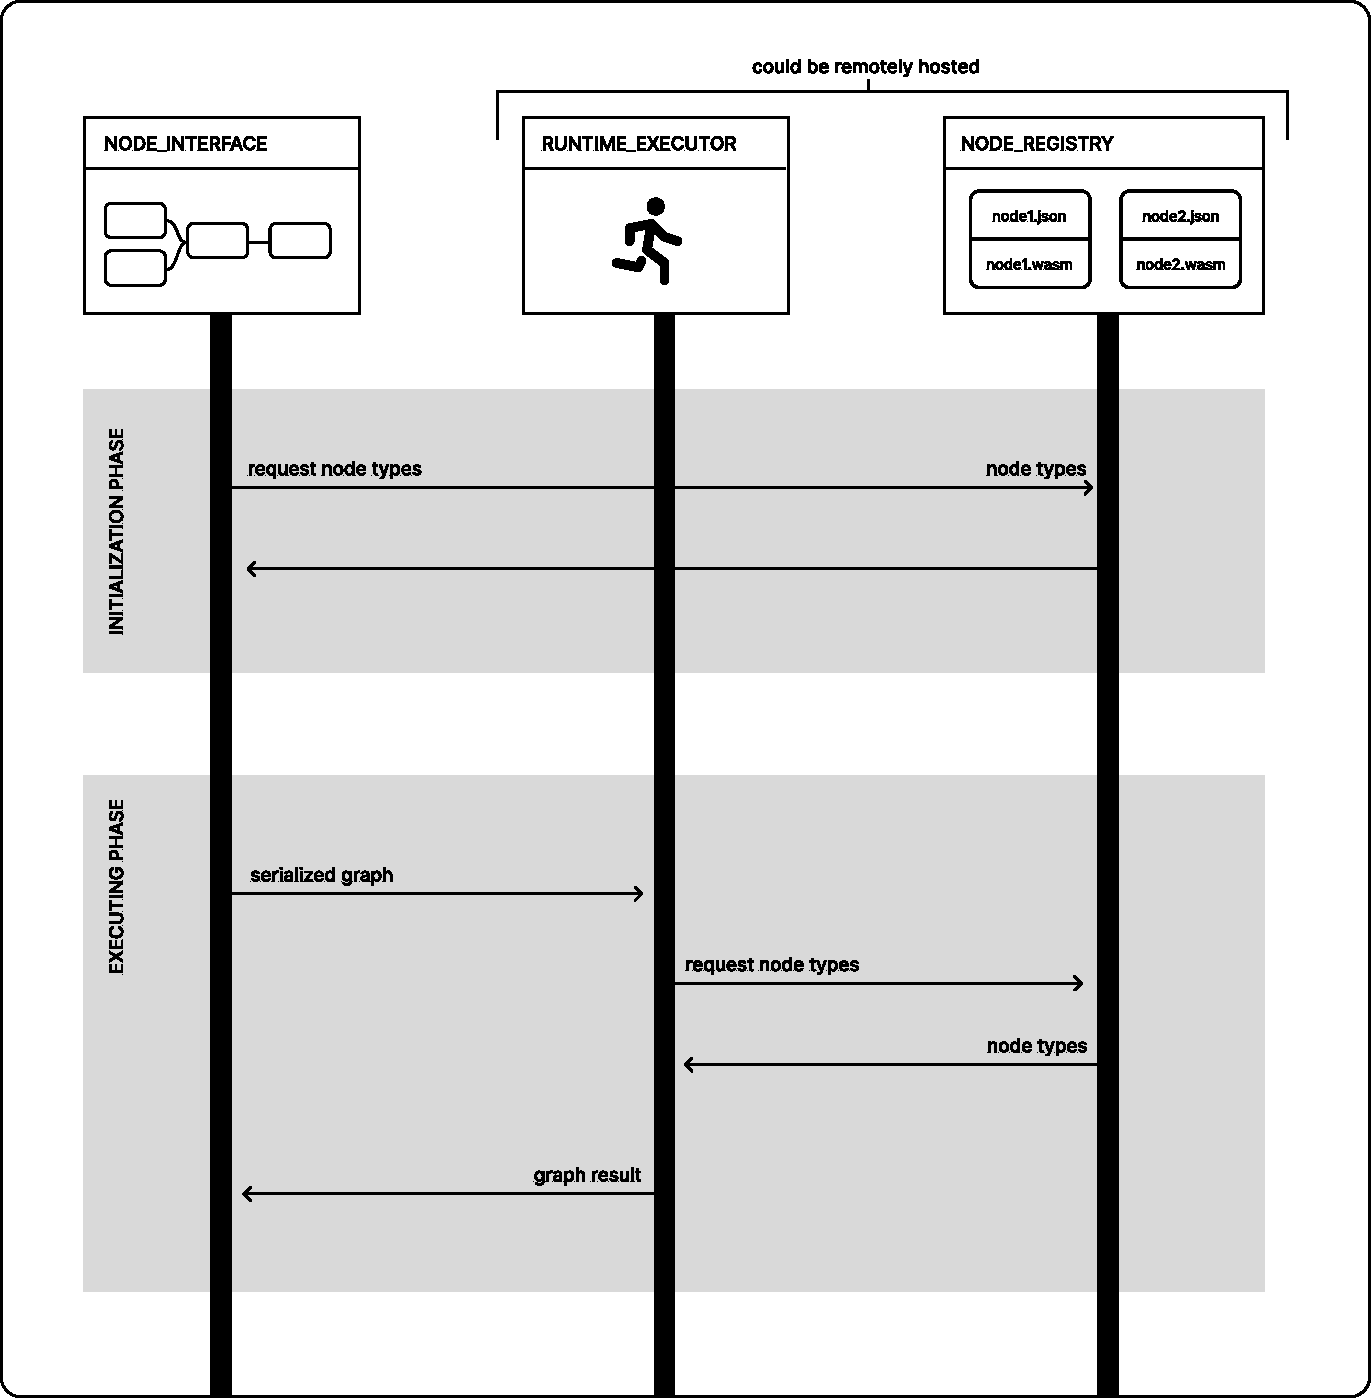
\includegraphics[width=0.8\textwidth]{graphics/OVERVIEW_SEQUENCE.pdf}
    \caption{Sequenzdiagramm der Architektur}
    \label{fig:your_label}
\end{figure}

\begin{figure}[htbp]
    \centering
    \begin{minipage}[b]{0.45\textwidth}
        \centering
        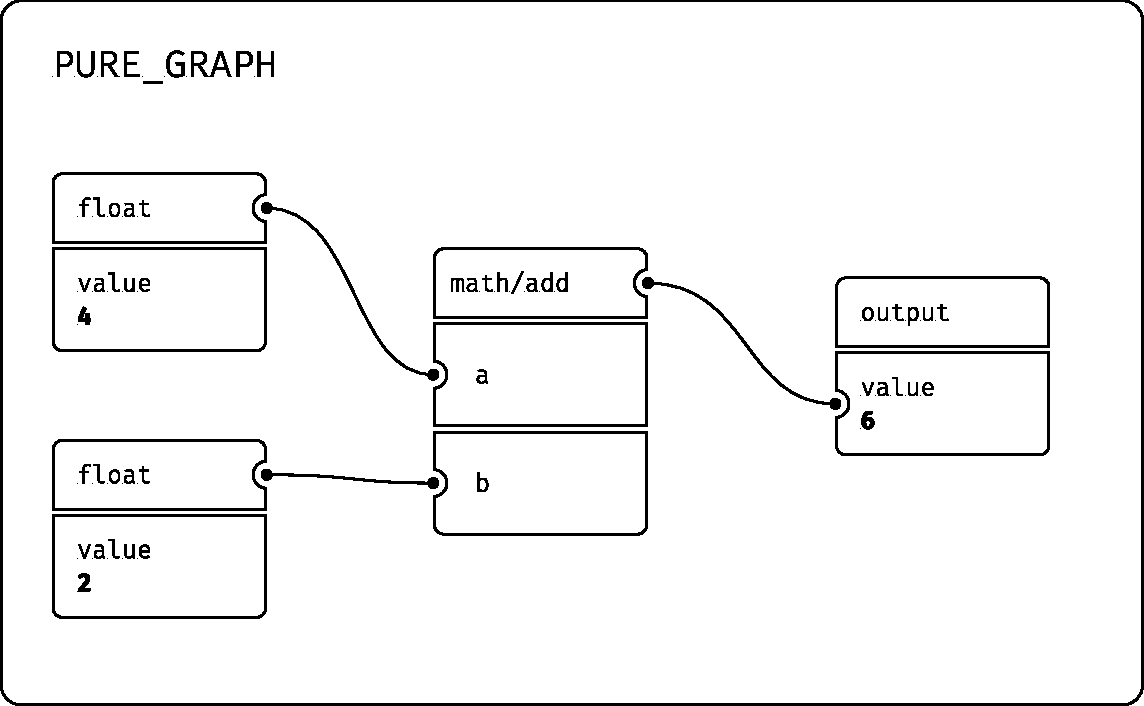
\includegraphics[width=\textwidth]{graphics/PURE_GRAPH.pdf}
        \caption{Darstellung eines \link{Node-Graph}}
        \label{sec:PURE_GRAPH}
    \end{minipage}
\end{figure}

\subsubsection{NODE\_INTERFACE}
\cmt{Visuelles Interface für den Node-Graph}
\subsubsection{NODE\_REGISTRY}
\cmt{Verwaltung der Nodes}
\subsubsection{RUNTIME\_EXECUTOR}
\cmt{Ausführung der Nodes}

\subsubsection{Higher Order Nodes / Parameter}
\label{sec:HON}
\cmt{Nodes die andere Nodes als Input oder Output haben}
\linebreak
\linebreak
In vorherigen Abschnitten wurden einzelne Nodes wie Funktionen besch
Es gibt Situationen, in denen es sinnvoll ist, von dem Konzept einer Node als reiner Funktion abzuweichen, die ihr Ergebnis berechnet und direkt an die nächste Node weitergibt.
\linebreak
\linebreak
Wie in Abbildung \ref{fig:random_problem} dargestellt, würde das Ergebnis der \topic{random} Node identisch sein, wenn sie nur einmal ausgeführt wird, unabhängig davon, wie viele \topic{math/add} Nodes als Empfänger dienen. 
Eine mögliche Lösung wäre, die \topic{random} Node für jede ihrer ausgehenden Verbindungen separat auszuführen. 
Dies könnte jedoch zur unnötigen Mehrfachausführung von Nodes führen, die dies nicht erfordern.
Außerdem erschwert dies das Caching von Node-Ergebnissen, da nicht nur die Node-Parameter, sondern auch die Anzahl der Verbindungen das Ergebnis beeinflussen würden.
\linebreak
\linebreak
Ein weiterer Nachteil ist das für dieses Konzept die Ausführung der Nodes nicht mehr nur in eine Richtung verläuft. Das könnte zu konzeptioneller Verwirrung und Komplexität führen.
\linebreak
\linebreak
\begin{figure}[htbp]
  \centering
  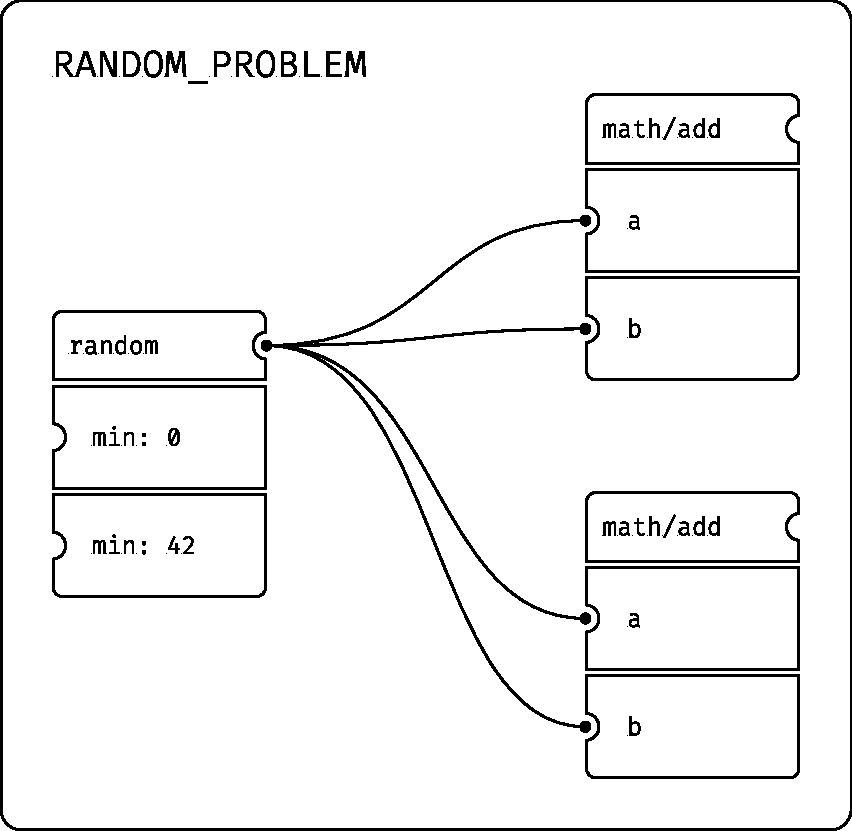
\includegraphics[width=0.5\textwidth]{graphics/RANDOM_PROBLEM.pdf}
  \caption{Illustration eines Problems mit der \texttt{random} Node}
  \label{fig:random_problem}
\end{figure}

\pagebreak

Ein weiteres Problem soll durch Abbildung \ref{fig:noise_problem} verdeutlicht werden.

\begin{figure}[htbp]
  \centering
  \includegraphics[width=0.8\textwidth]{./graphics/NOISE_PROBLEM.pdf}
  \caption{Problemdarstellung}
  \label{fig:noise_problem}
\end{figure}

\subsection{Technologien}
\subsubsection{Svelte}
\subsubsection{Rust}
\subsection{Design}

\section{Implementierung}
\subsection{UI}
\subsection{Backend}

\section{Evaluation}
\section{Fazit}

\pagebreak
\section{Glossar}

\subsection{Node}
\label{sec:Node}
Einzelner Baustein eines \hyperref[sec:Node-Graph]{Node-Graphs}. Eine Node funktioniert etwa wie eine Funktion in einer textuellen Programmiersprache. Sie nimmt \hyperref[sec:Node-Argumente]{Node-Argumente} entgegen, verarbeitet diese und gibt ein Ergebnis zurück. 

\begin{figure}[htbp]
    \centering
    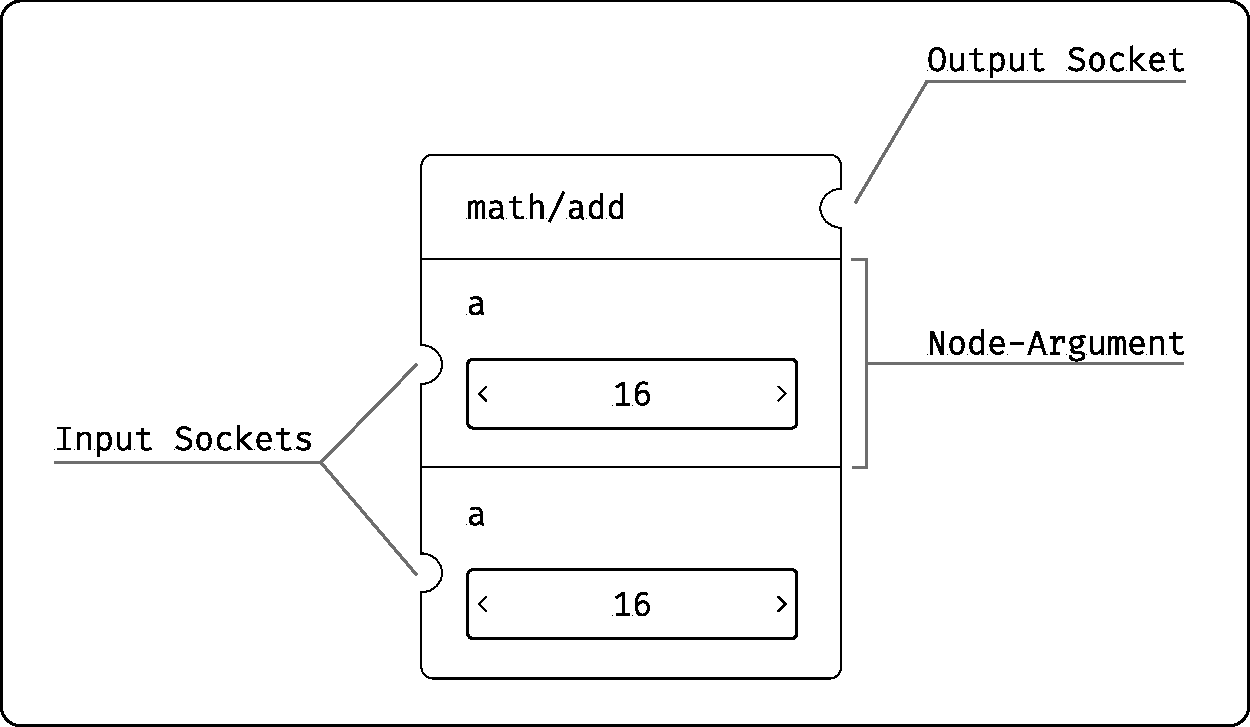
\includegraphics[width=0.8\textwidth]{graphics/NODE_ANATOMY.pdf}
    \caption{Anatomie einer Node}
    \label{sec:NODE_ANATOMY}
\end{figure}

\subsection{Node-Typ}
\label{sec:Node-Typ}
Eine Node ist quasi eine Instanz eines Node-Typs. Ein Node-Typ definiert die Struktur einer Node. Er enthält Informationen über die Inputs und Outputs einer Node und die Funktion, die die Node ausführt.

\subsection{Node-Graph}
\label{sec:Node-Graph}
Node-Graphs sind ein gerichteter \link[PURE_GRAPH]{azyklischer Graph (DAG)} von \hyperref[sec:Node]{Nodes}. Sie bestehen aus einer Menge von Nodes und deren Verknüpfungen. 

\subsection{Node-Argumente}
\label{sec:Node-Argumente}
Node-Argumente sind die Eingabeparameter einer Node. Ein Node-Argument kann entweder direkt über das Interface in einer \hyperref[sec:Node]{Node} definiert werden oder indem der User einen Output-Socket einer anderen Node mit dem \link{Node-Socket} eines Node-Argument verknüpft.

\subsection{Node-Socket}
\label{sec:Node-Socket}
Node-Sockets sind die Verbindungspunkte zwischen \link[Node]{Nodes}. Eine Node hat mehrere Input-Sockets und einen Output Socket.


\pagebreak
\section{Literaturverzeichnis}

\printbibliography

\end{document}
